% id: 0326
% book: RPM 기하 · 03 공간도형
% section: 시험에 꼭 나오는 문제
% figure: crop:fig-0326.png
% answer: $6$
% answer_source: 답지
% variant_level: 0 (원본 전사)
% 이 파일은 build.mjs 가 items.json 에서 만든다. 고칠 때는 items.json 을 고친다.
\smash{\raisebox{1.5mm}{\dmkichul{RPM 기하 0326번 · 53쪽}}}
\noindent\begin{minipage}[t]{0.58\linewidth}\vspace{0pt}\raggedright 오른쪽 그림과 같은 사각뿔에서 네 꼭짓점~$\pt{B}$, $\pt{C}$, $\pt{D}$, $\pt{E}$와 두 직선~$\pt{AC}$, $\pt{AE}$로 만들 수 있는 서로 다른 평면의 개수를 구하시오.\end{minipage}\hfill\begin{minipage}[t]{0.4\linewidth}\vspace{0pt}\centering \setlength{\dmfigw}{88.5pt}\ifdim\dmfigw>\linewidth\setlength{\dmfigw}{\linewidth}\fi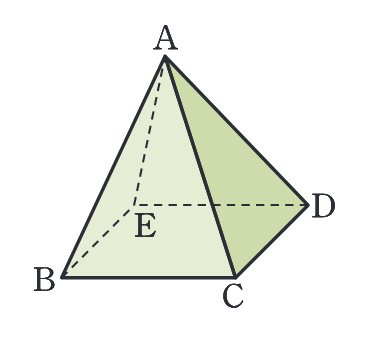
\includegraphics[width=\dmfigw]{figures/fig-0326.png}\end{minipage}\par
